
%----------------------------------------------------------------------------------------
%   Хавсралтууд эндээс эхэлнэ
%----------------------------------------------------------------------------------------
\appendix
\addcontentsline{toc}{part}{ХАВСРАЛТ}

\chapter{Кодын хэрэгжүүлэлт}
\section{Системийн хэсэг}
\subsection{BinarySpaceTree}
\begin{lstlisting}[language={[Sharp]C}, frame=single, caption=BinarySpaceTree хэрэгжүүлэлт]
using System.Collections.Generic;
using System.Data;
using System.Linq;
using System.Text;
using CodeMonkey.Utils;
using Unity.VisualScripting;
using UnityEngine;
using UnityEngine.Rendering.UI;
using Random = UnityEngine.Random;


namespace DefaultNamespace
{
    public class BinarySpaceTree
    {
        public static int VERTICAL_CUT_INDEX = 0;
        public static int HORIZONTAL_CUT_INDEX = 1;

        private Rectangle _nodeRectangle;
        private BinarySpaceTree _leftChild;
        private BinarySpaceTree _rightChild;
        private BinarySpaceTree _parentCell;
        private bool _isLeaf = true;
        private int _level = 0;
        private ProceduralGenerationCellBundle _bundle;
        public int Key;

        public Rectangle NodeRectangle
        {
            get => _nodeRectangle;
            set => _nodeRectangle = value;
        }


        public bool IsLeaf => _isLeaf;

        public int Level => _level;

        public BinarySpaceTree RightChild
        {
            get => _rightChild;
            set
            {
                if (value == null)
                    return;
                _rightChild = value;
                _isLeaf = false;
            }
        }

        public BinarySpaceTree LeftChild
        {
            get => _leftChild;
            set
            {
                if (value == null)
                    return;
                _leftChild = value;
                _isLeaf = false;
            }
        }

        public BinarySpaceTree ParentCell
        {
            get => _parentCell;
            set
            {
                if (value == null)
                {
                    _parentCell = null;
                    _level = 0;
                }
                else
                {
                    _parentCell = value;
                    _level = _parentCell._level + 1;
                }
            }
        }


        public BinarySpaceTree(Rectangle nodeRectangle, ProceduralGenerationCellBundle bundle)
        {
            NodeRectangle = nodeRectangle;
            _bundle = bundle;
            ParentCell = null;
            Key = 1;
            Divide();
        }

        private BinarySpaceTree(Rectangle nodeRectangle, BinarySpaceTree parentCell,
            ProceduralGenerationCellBundle bundle, int key)
        {
            NodeRectangle = nodeRectangle;
            ParentCell = parentCell;
            _bundle = bundle;
            Key = key;
            Divide();
        }

        public void Divide()
        {
            if (CanMutateToBeBig()) return;
            int direction = GetDirectionToCut();
            if (direction == -1) return;
            CreateChildNodes(direction);
        }

        private void CreateChildNodes(int direction)
        {
            if (direction == VERTICAL_CUT_INDEX)
            {
                CreateChildNodesVertically();
            }
            else
            {
                CreateChildNodesHorizontally();
            }
        }

        private void CreateChildNodesHorizontally()
        {
            var divisionAmount = Random.Range(_bundle.MIN_ROOM_SIZE, NodeRectangle.Height + 1 - _bundle.MIN_ROOM_SIZE);
            divisionAmount = Math.Max(_bundle.MIN_ROOM_SIZE, divisionAmount);

            var leftChildCoords2D = new Coord2D(NodeRectangle.StartingCoord2D.X, NodeRectangle.StartingCoord2D.Z);
            var leftChildRectangle = new Rectangle(leftChildCoords2D, NodeRectangle.Width, divisionAmount);
            LeftChild = new BinarySpaceTree(leftChildRectangle, this, _bundle, Key * 2);

            var rightChildCoords2D = new Coord2D(NodeRectangle.StartingCoord2D.X,
                NodeRectangle.StartingCoord2D.Z + divisionAmount);
            var rightChildRectangle = new Rectangle(rightChildCoords2D, NodeRectangle.Width,
                NodeRectangle.Height - divisionAmount);
            RightChild = new BinarySpaceTree(rightChildRectangle, this, _bundle, Key * 2 + 1);
        }

        private void CreateChildNodesVertically()
        {
            var divisionAmount = Random.Range(_bundle.MIN_ROOM_SIZE, NodeRectangle.Width + 1 - _bundle.MIN_ROOM_SIZE);
            divisionAmount = Math.Max(_bundle.MIN_ROOM_SIZE, divisionAmount);

            var leftChildCoords2D = new Coord2D(NodeRectangle.StartingCoord2D.X, NodeRectangle.StartingCoord2D.Z);
            var leftChildRectangle = new Rectangle(leftChildCoords2D, divisionAmount, NodeRectangle.Height);
            LeftChild = new BinarySpaceTree(leftChildRectangle, this, _bundle, Key * 2);

            var rightChildCoords2D = new Coord2D(NodeRectangle.StartingCoord2D.X + divisionAmount,
                NodeRectangle.StartingCoord2D.Z);
            var rightChildRectangle = new Rectangle(rightChildCoords2D, NodeRectangle.Width - divisionAmount,
                NodeRectangle.Height);
            RightChild = new BinarySpaceTree(rightChildRectangle, this, _bundle, Key * 2 + 1);
        }

        private int GetDirectionToCut()
        {
            int direction;
            if (NodeRectangle.Width >= _bundle.MIN_ROOM_SIZE * 2 && NodeRectangle.Height < _bundle.MIN_ROOM_SIZE * 2)
                direction = VERTICAL_CUT_INDEX;
            else if (NodeRectangle.Width < _bundle.MIN_ROOM_SIZE * 2 &&
                     NodeRectangle.Height >= _bundle.MIN_ROOM_SIZE * 2)
                direction = HORIZONTAL_CUT_INDEX;
            else if (NodeRectangle.Width >= _bundle.MIN_ROOM_SIZE * 2 &&
                     NodeRectangle.Height >= _bundle.MIN_ROOM_SIZE * 2)
                direction = Random.Range(0, 2);
            else
                return -1;
            return direction;
        }

        private bool CanMutateToBeBig()
        {
            if (_level == 0) return false;
            if (NodeRectangle.Width < _bundle.MAX_ROOM_SIZE && NodeRectangle.Height < _bundle.MAX_ROOM_SIZE)
            {
                // multiplying because the generator has 0.5 chance multiplier
                // max bundle leaf node input is 50, so max is 50%
                if (RandomUtils.Chance(_bundle.LEAF_NODE_CHANCE * 2))
                    return true;
            }

            return false;
        }

        public void AssignNodesAtLevelFromRootNode(int level, List<BinarySpaceTree> nodesAtLevel)
        {
            if (Key != 1)
                throw new InvalidOperationException("This is not the root node");
            AssignNodesAtLevelForNode(level, nodesAtLevel);
        }

        private void AssignNodesAtLevelForNode(int level, List<BinarySpaceTree> nodesAtLevel)
        {
            if (Level == level)
            {
                nodesAtLevel.Add(this);
            }

            if (LeftChild != null)
                LeftChild.AssignNodesAtLevelForNode(level, nodesAtLevel);
            if (RightChild != null)
                RightChild.AssignNodesAtLevelForNode(level, nodesAtLevel);
        }


        public void AssignLeafNodesFromRootNode(List<BinarySpaceTree> leafNodes)
        {
            if (Key != 1)
                throw new InvalidOperationException("This is not the root node");
            AssignLeafNodes(leafNodes);
        }

        private void AssignLeafNodes(List<BinarySpaceTree> leafNodes)
        {
            if (IsLeaf)
            {
                leafNodes.Add(this);
                return;
            }

            LeftChild.AssignLeafNodes(leafNodes);
            RightChild.AssignLeafNodes(leafNodes);
        }

        public BinarySpaceTree GetSibling()
        {
            if (ParentCell == null)
                throw new InvalidOperationException("This node doesn't have a parent");
            if (Key != ParentCell.LeftChild.Key)
                return ParentCell.LeftChild;

            return ParentCell.RightChild;
        }

        public bool IsRightChild()
        {
            if (ParentCell == null)
                throw new InvalidOperationException("This node doesn't have a parent");
            if (ParentCell.RightChild.Key == Key)
            {
                return true;
            }

            return false;
        }

        public static int GetLevelDepth(BinarySpaceTree binarySpaceTree, int initialLevel = 1)

        {
            if (binarySpaceTree.Key != 1)
                throw new InvalidOperationException("This is not the root node");

            List<BinarySpaceTree> nodesAtTheBottom = new List<BinarySpaceTree>();
            binarySpaceTree.AssignLeafNodes(nodesAtTheBottom);

            nodesAtTheBottom.ForEach(e =>
            {
                if (e.Level > initialLevel)
                {
                    initialLevel = e.Level;
                }
            });
            return initialLevel;
        }


        public BinarySpaceTree GetNodesAtIndex(int index)
        {
            if (this.Key != 1)
                throw new InvalidOperationException("This is not the root node");
            return GetNodeAtIndexHelper(this, index);
        }

        // in-order traversal
        private static BinarySpaceTree GetNodeAtIndexHelper(BinarySpaceTree node, int index)
        {
            if (node == null)
                return null;

            if (node.Key == index)
                return node;
            BinarySpaceTree leftNode = GetNodeAtIndexHelper(node.LeftChild, index);

            if (leftNode != null)
            {
                if (leftNode.Key == index)
                    return leftNode;
            }

            return GetNodeAtIndexHelper(node.RightChild, index);
        }

        public static void InorderTraversalDebugLog(BinarySpaceTree root)
        {
            if (root != null)
            {
                InorderTraversalDebugLog(root.LeftChild);
                Debug.Log(root.Key + " ");
                InorderTraversalDebugLog(root.RightChild);
            }
        }

        public Coord2D GetStartingCoords()
        {
            return NodeRectangle.StartingCoord2D;
        }
    }
}
\end{lstlisting}
\chapter{Ажлын төлөвлөгөө}
\begin{figure}[b]
	\centering
	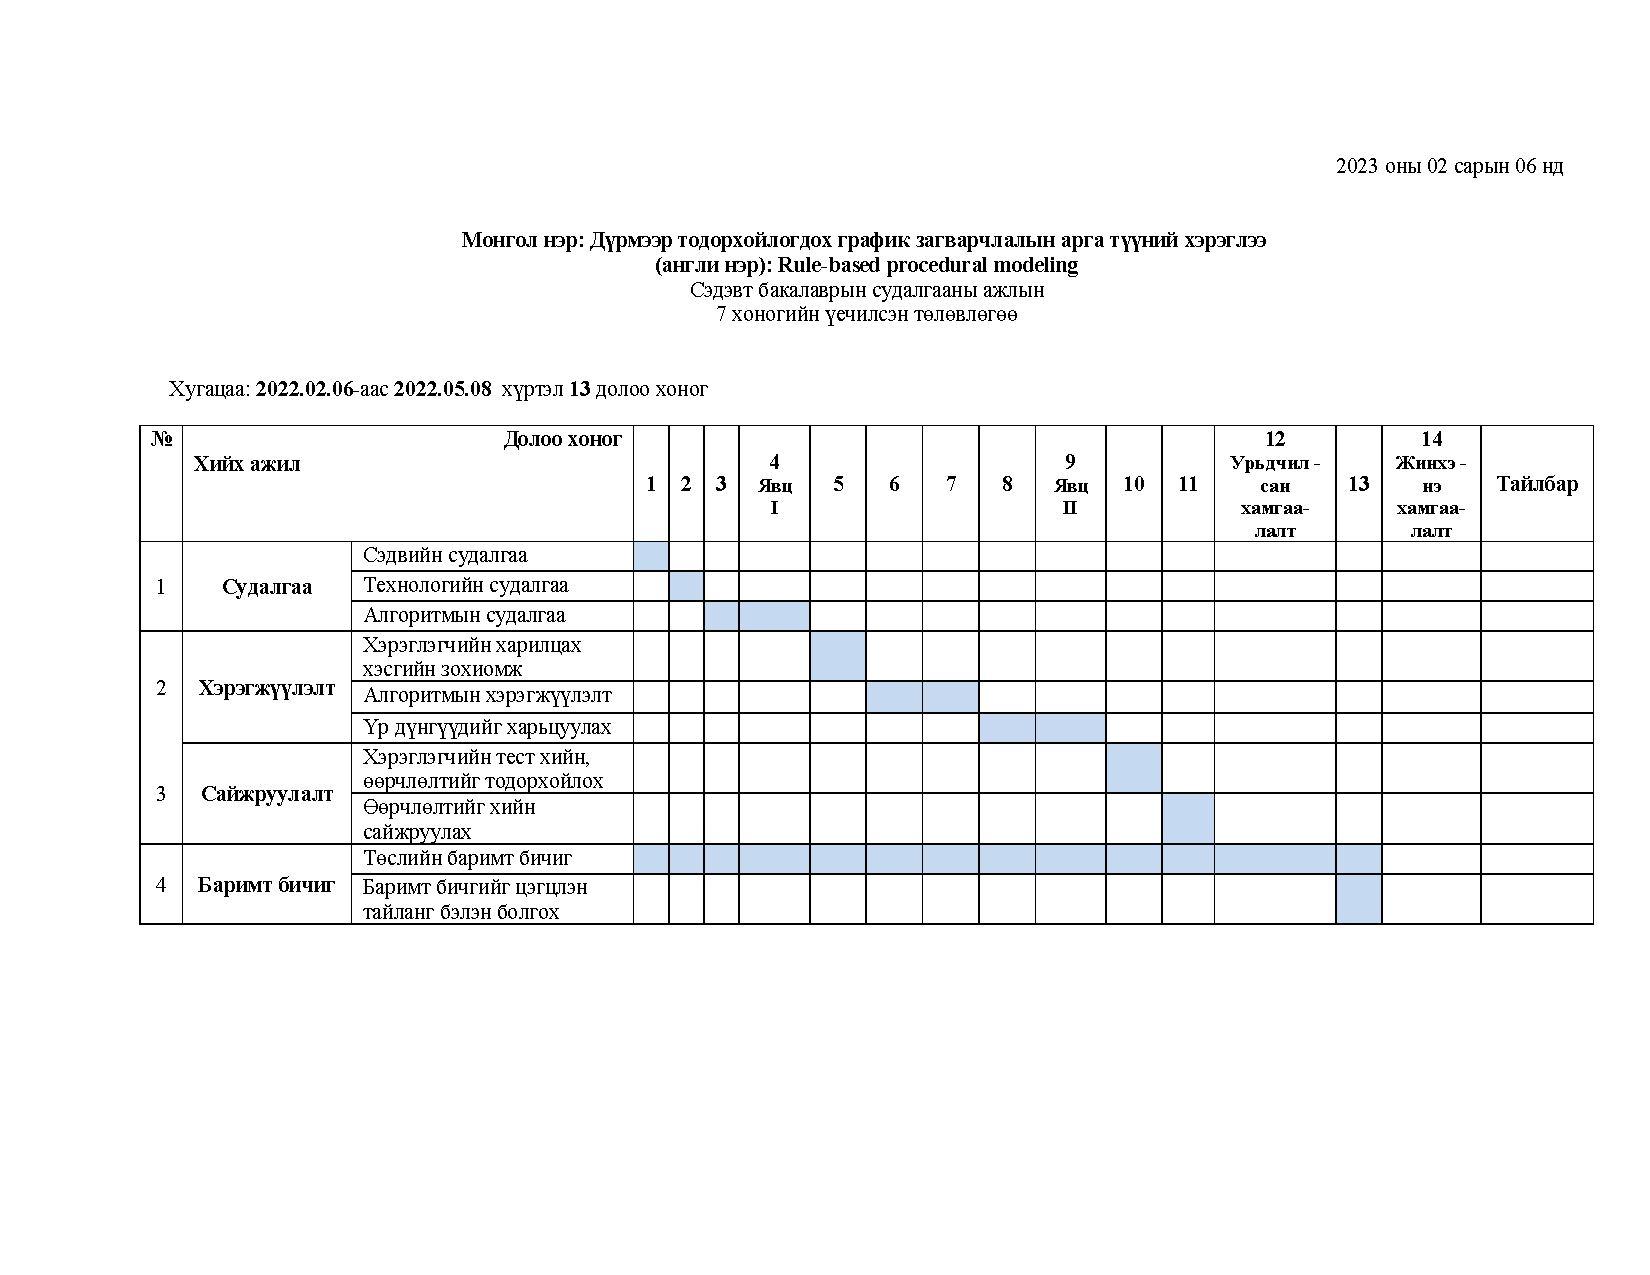
\includegraphics[angle=90,height=\textheight]{./images/plan.pdf}
	\caption{Ажлын төлөвлөгөө}
	\label{fig:WorkPlan}
\end{figure}